\section*{Background and Evolution of Threat Modeling}
Threat modeling is the systematic analysis of potential threats to information systems, with the goal of identifying, quantifying, and mitigating security risks\cite{shostack2014,uceda2015}. This chapter traces the evolution of threat modeling from early security practices to the modern, multi-framework discipline it is today.

\subsection*{Early Security Practices}
In the early days of computing, security was largely perimeter-based, relying on firewalls, access controls, and antivirus software. The focus was on keeping external attackers out, with little attention to insider threats or application-level vulnerabilities\cite{schneier1999}. Security was often reactive, responding to incidents rather than proactively identifying risks.

\subsection*{The Rise of Structured Threat Modeling}
By the late 1990s, the complexity of software systems and the sophistication of attackers demanded a more systematic approach. Microsoft introduced the STRIDE framework\cite{shostack2014}, which provided a repeatable process for identifying threats during software design. Academic and industry researchers developed additional models, such as OCTAVE (Carnegie Mellon) and PASTA\cite{uceda2015}, recognizing that security is both a technical and business concern.

\subsection*{Key Milestones and Timeline}
\begin{itemize}
	\item \textbf{1999: STRIDE} — Microsoft introduces STRIDE, categorizing threats into six types and integrating threat modeling into the Secure Development Lifecycle (SDL)\cite{shostack2014}.
	\item \textbf{2001: OCTAVE} — Carnegie Mellon University develops OCTAVE, focusing on organizational risk and asset-based analysis.
	\item \textbf{2012: PASTA} — The Process for Attack Simulation and Threat Analysis (PASTA) is published, emphasizing attacker perspective and business impact\cite{uceda2015}.
	\item \textbf{2010s: VAST, Trike, and OWASP} — New frameworks emerge to address scalability, risk quantification, and agile development needs\cite{owasp}.
\end{itemize}

\begin{figure}[H]
	\centering
	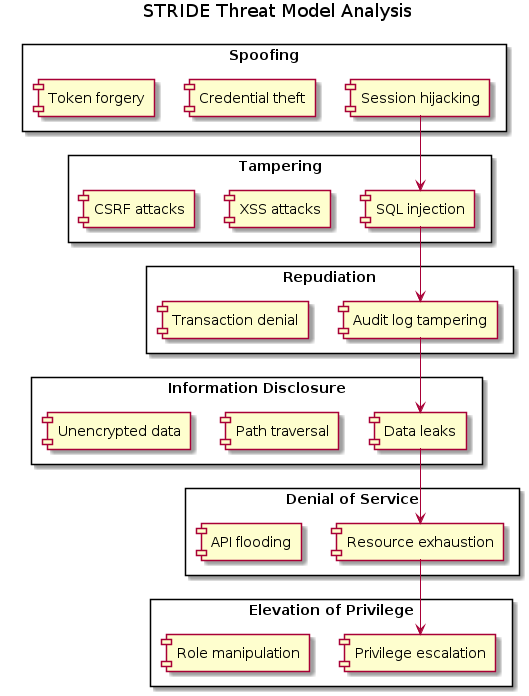
\includegraphics[width=0.8\textwidth]{images/stride-analysis}
	\caption{Timeline of Major Threat Modeling Frameworks}
\end{figure}

\subsection*{Modern Threat Modeling}
Today, threat modeling is a mature discipline, supported by a wide range of tools, methodologies, and community resources. It is recognized as a best practice by standards bodies (NIST SP 800-154\cite{nist800154}, ISO 27001), regulatory frameworks (GDPR, HIPAA), and industry groups (OWASP\cite{owasp}). Modern threat modeling addresses not only technical vulnerabilities, but also business logic, supply chain risks, and emerging technologies such as cloud, IoT, and AI.

\subsection*{Summary}
The evolution of threat modeling reflects the growing complexity of information systems and the need for proactive, structured security analysis. Today’s best practices are grounded in decades of research and real-world experience, as documented in leading books and standards\cite{shostack2014,uceda2015,owasp,nist800154,schneier1999}.
